\chapter{基于扩散模型的模仿学习动作生成算法}
\label{chp:diffusion_action_generation}

在机械臂操作任务中，由于环境的复杂性和任务的多样性，同一任务往往存在多条合理的操作路径，这种现象导致专家示教数据中的动作分布呈现出明显的多模态特性。传统的行为克隆方法通常假设动作分布是单峰的，倾向于将多种可能的动作轨迹平均化，这在面临多模态分布时容易产生无效甚至危险的动作指令。为了解决这一问题，本章提出一种基于扩散模型的模仿学习动作生成算法，利用扩散模型对复杂数据分布的拟合能力，提升动作策略在非结构化环境中的适应性和鲁棒性，并在机器人操作数据集RoboMimic\cite{mandlekar2021matters}上进行验证。

\section{扩散动作生成算法}
\label{sec:diffusion_action_architecture}

基于扩散模型的模仿学习动作生成算法的核心在于构建一个能够融合多模态感知信息并输出连续动作序列的条件生成模型。该算法的整体架构如图\ref{fig:action_model}所示，主要由特征编码器、特征融合模块和扩散动作生成模块三部分组成。

\begin{figure}[htbp]
  \centering
  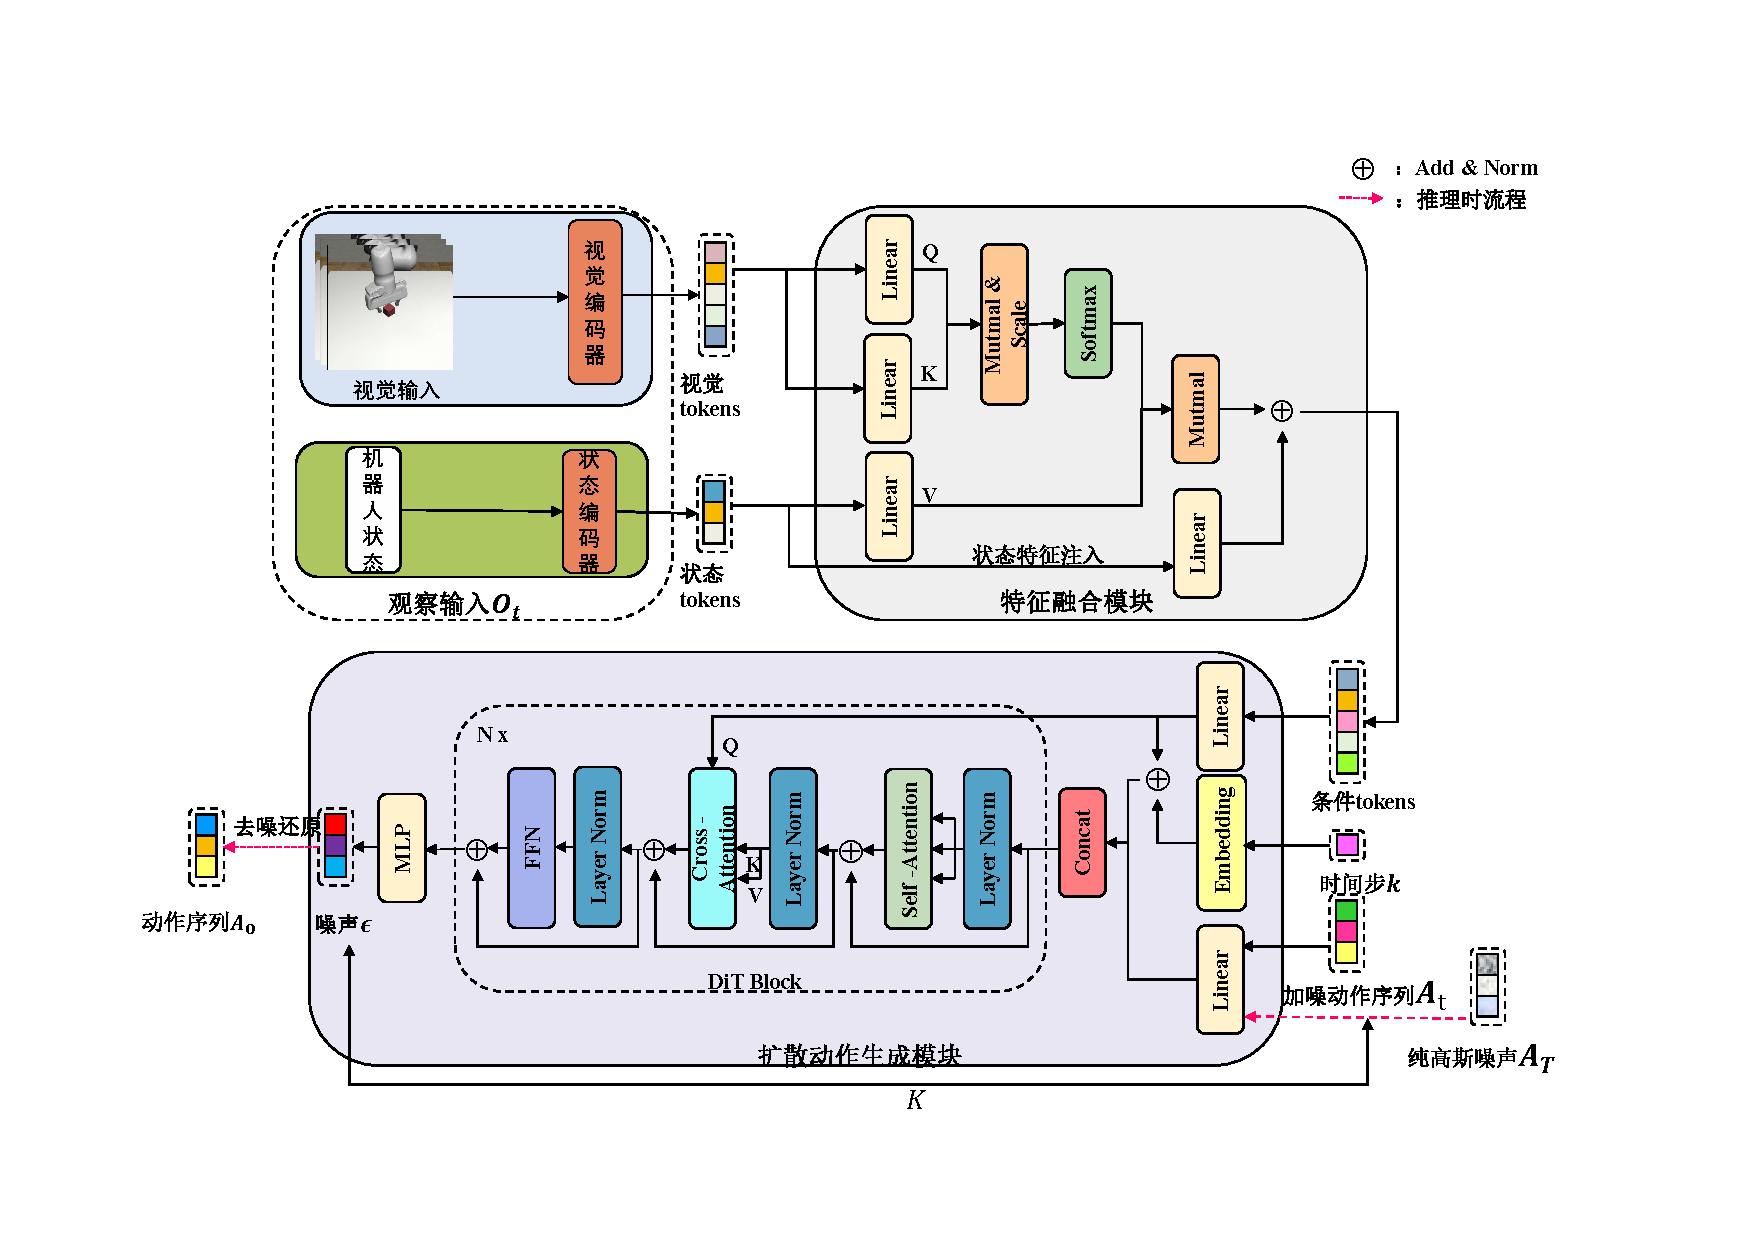
\includegraphics[width=0.88\linewidth]{figures/content/action_model}
  \caption{基于扩散模型的模仿学习动作生成算法整体架构}
  \label{fig:action_model}
\end{figure}

系统首先接收来自环境的观察输入 $O_t$，该输入包含视觉输入和机器人状态两部分，视觉输入通过视觉编码器提取为视觉特征表示，而机器人当前关节角度、末端执行器位姿等状态，则通过状态编码器转化为状态特征表示。这两种特征表示在特征融合模块中进行交互与整合，以形成统一的条件特征,为后续的动作生成提供充分的环境与自身状态上下文。

扩散动作生成模块负责基于上述条件特征生成连续的动作序列 $A_0$,该模块采用基于Transformer架构的扩散模型（DiT）\cite{peebles2023scalable}作为核心去噪网络，DiT网络由多个堆叠的DiT Block组成，用于逐步预测输入序列中的噪声 $\epsilon$。在训练阶段，模型接收添加了噪声的动作序列 $A_t$、当前时间步 $k$ 以及条件特征作为输入。在推理阶段，模型从纯高斯噪声出发，在条件特征的引导下，经过多步迭代去噪，最终生成符合专家分布的干净动作序列 $A_0$，并下发给机械臂执行。

\subsection{视觉与状态特征编码}
\label{sec:visual_state_encoding}
在本文提出的基于扩散模型的动作生成算法中，模型需要结合多步的历史观察序列来预测未来的动作序列。由于每一时间步的视觉观测都需要经过编码器处理，计算延迟和显存占用会随着观察窗口步数的增加而线性增长。如果在视觉编码阶段产生过高的延迟或占用过多的显存，将严重制约整个动作生成算法的实时性。为了在保证特征提取质量的同时满足机械臂实时控制对推理速度的要求，本算法采用EfficientViT\cite{cai2023efficientvit}作为视觉编码器的骨干网络，传统的视觉Transformer通常依赖于标准的Softmax自注意力机制来获取全局感受野，但其计算复杂度和显存消耗与输入图像分辨率的平方成正比。这在处理高分辨率的多帧图像序列时，会带来不可接受的计算负担。EfficientViT通过引入多尺度线性注意力机制，在保持全局感受野和多尺度学习能力的同时，降低了计算复杂度和内存消耗，从而能够契合了本算法对高效视觉编码的需求。


\begin{figure}[htbp]
  \centering
  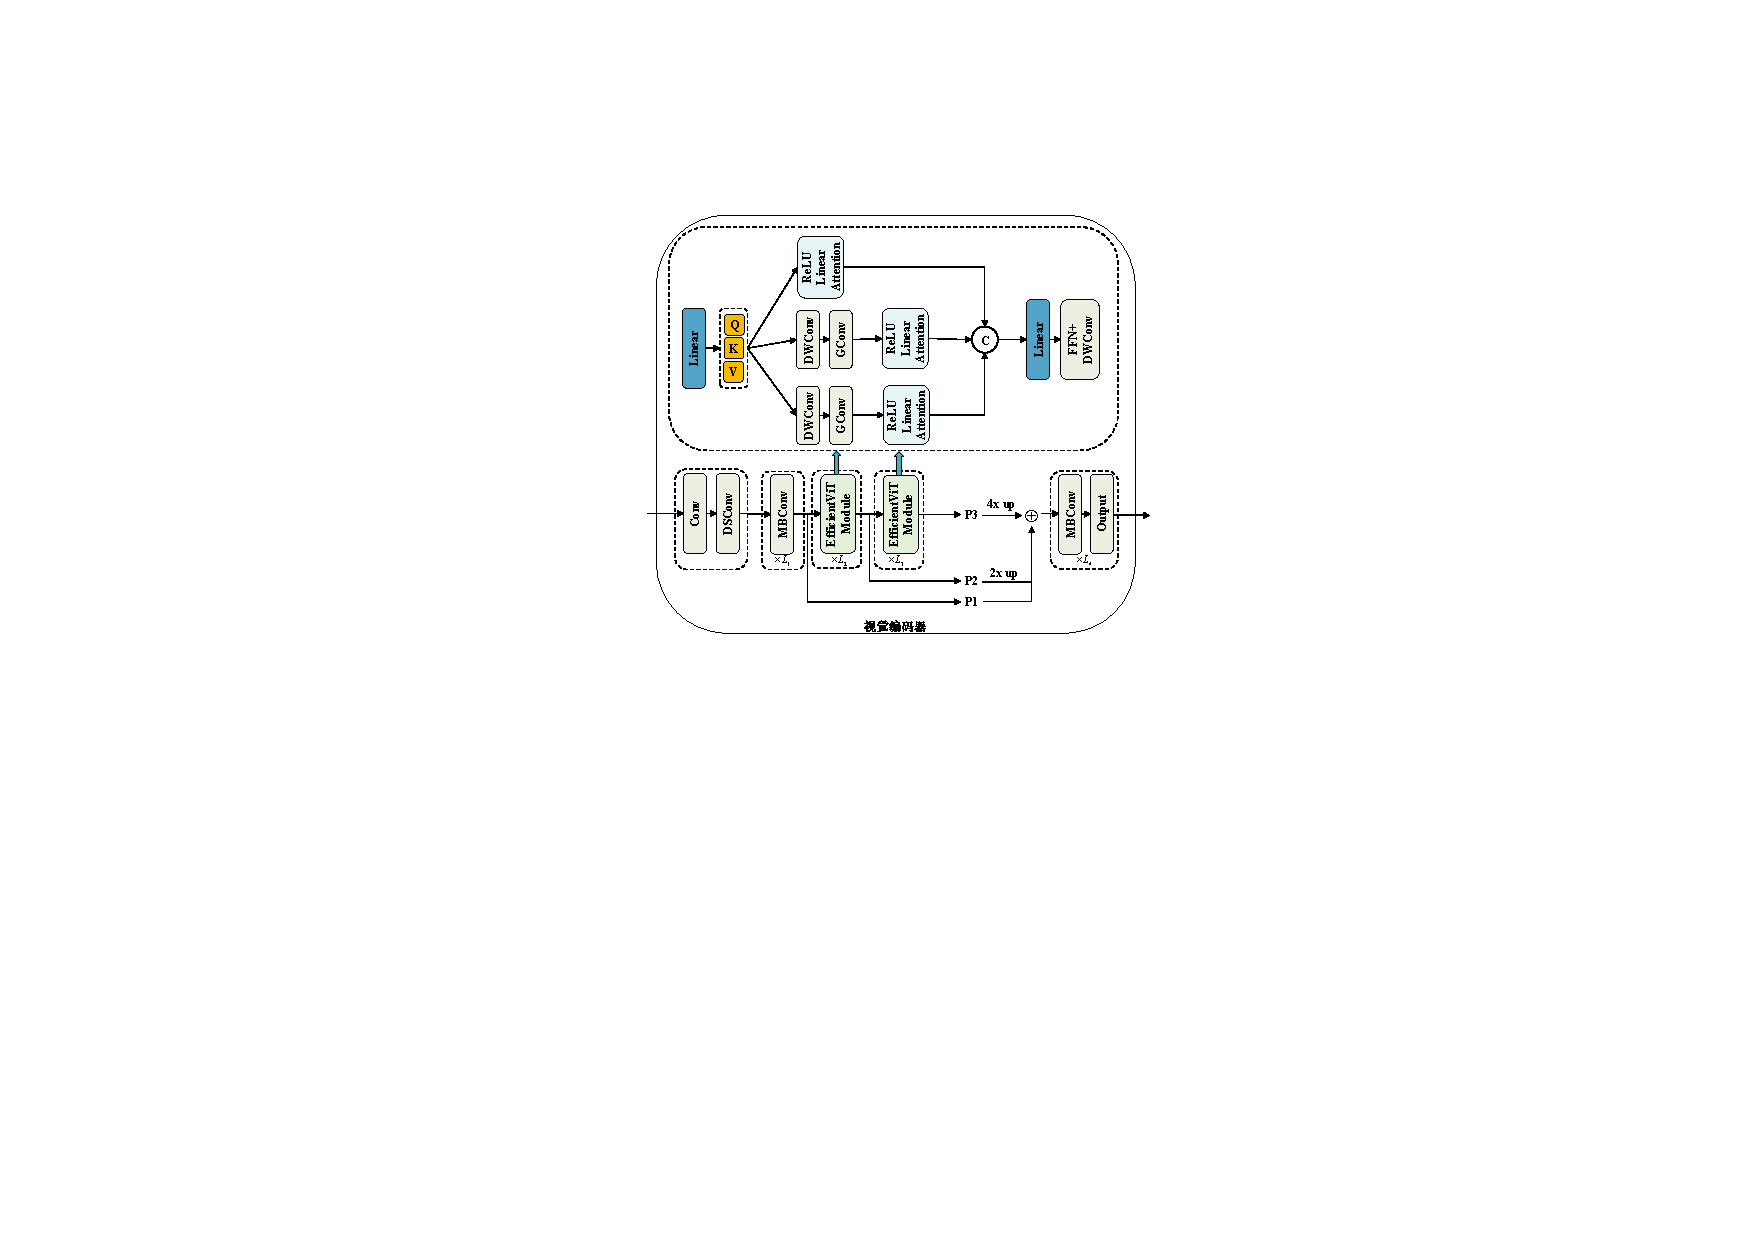
\includegraphics[width=0.8\linewidth]{figures/content/efficent_vit}
  \caption{EfficientViT视觉编码器网络结构}
  \label{fig:efficient_vit}
\end{figure}

如图\ref{fig:efficient_vit}所示，EfficientViT视觉编码器通过多阶段的网络结构对输入图像进行层次化的特征提取。网络设计中广泛采用了轻量化卷积操作，其中DSConv表示深度可分离卷积，MBConv表示移动翻转瓶颈卷积，DWConv表示深度卷积，GConv表示组卷积。在初始阶段，输入图像经过普通卷积和深度可分离卷积进行初步的下采样和特征提取。随后，特征图进入包含EfficientViT模块的核心处理阶段。

EfficientViT模块内部采用轻量级的多尺度注意力机制，特征首先经过线性层映射为Q、K和V向量。为了克服传统线性注意力在局部信息提取上的不足，模块利用不同分组的深度可分离卷积和组卷积对Q、K、V向量进行局部聚合，生成多尺度特征表示。随后，模块采用ReLU激活函数替代传统的Softmax函数进行注意力计算，通过利用矩阵乘法的结合律，ReLU线性注意力将计算顺序从先计算注意力权重矩阵转变为先计算键和值的乘积，从而将计算复杂度从与分辨率的平方级关系降低为线性关系。此外，使用ReLU替代Softmax避免了在硬件上执行效率低下的行归一化操作，大幅提升了内存访问效率。

多尺度注意力图在通道维度上进行拼接后，再通过线性层进行特征融合。同时，网络在不同阶段之间引入了上采样操作，以便在不同分辨率层级之间进行特征融合，从而捕获丰富的空间细节和全局语义信息。这种机制上的协同配合，使得EfficientViT在提取高质量视觉特征的同时，大幅降低了多步观察序列带来的显存压力和计算延迟。最终，视觉编码器输出一组具有高表征能力的视觉特征向量，用于后续的特征融合与动作生成。

对于机器人状态编码，由于各关节的当前角度、末端执行器位姿和夹爪的开合状态这样的状态数据通常是低维向量，可直接采用多层感知机（MLP）作为状态编码器，如图\ref{fig:state_encoder}。该编码器由两个全连接层和GeLU激活函数组成，负责将低维的原始状态向量映射到与视觉特征相同维度的高维潜在空间中，并通过Position Embedding得到状态向量，以便在特征融合模块中与视觉特征进行有效的交互和对齐。
\begin{figure}[htbp]
  \centering
  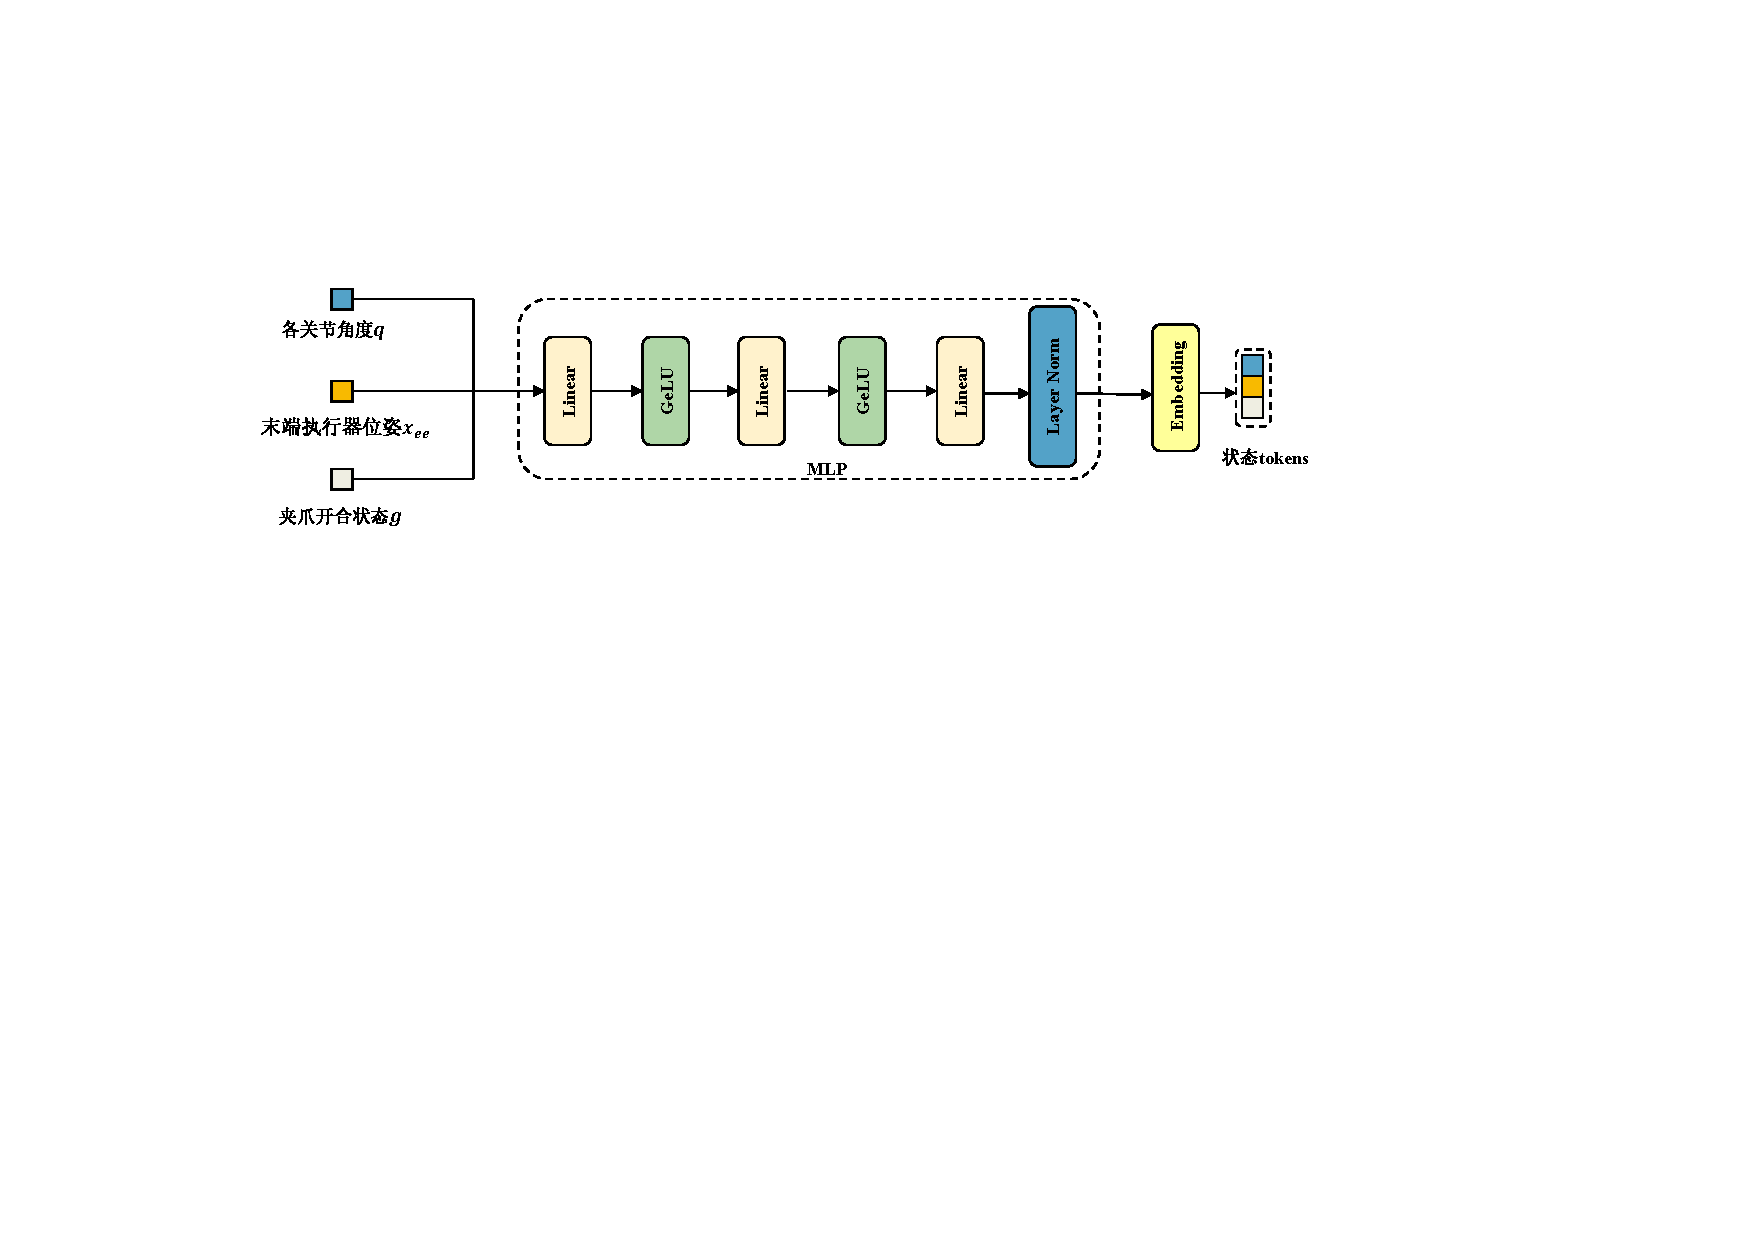
\includegraphics[width=0.66\linewidth]{figures/content/state_encoder}
  \caption{状态编码器结构示意图}
  \label{fig:state_encoder}
\end{figure}


